\documentclass[10pt,a4paper]{report}
\usepackage[utf8]{inputenc}
\usepackage[T1]{fontenc}
\usepackage{graphicx}
\usepackage{amsmath}
\usepackage{float}
\usepackage{xfrac}
\usepackage[pdfpagelabels]{hyperref}
\setlength{\parskip}{1em}

%opening
\title{MDFourier}
\author{Artemio Urbina}

\begin{document}

\pagenumbering{Alph}
\begin{titlepage}
	\maketitle
	\thispagestyle{empty}
\end{titlepage}
\pagenumbering{arabic}

\tableofcontents

\chapter{MDFourier Objective}

Provide a Fourier based analysis framework to compare audio generated by any \textit{Mega Drive/Genesis} variant, clone or implementation. This is of course not limited to one specific system, and the software can be used to compare any other platform with new configuration files.

The intention is not to disparage any particular implementation, but help to understand and improve them whenever possible by identifying the differences. This can help emulators, \textit{FPGA} implementations and even hardware modifications to better match the desired reference profile.

\section{What is it for?}

It can be used to identify the differences between two audio signatures. These can come from iterations of the console family, like a \textit{Sega Genesis Model 1 VA3} and a \textit{Sega Model 2 VA 1.8}, or even between a console and a hardware modification, recapping the system, an emulator, or an \textit{FPGA} implementation.

These results can be used to determine if the signals are indeed different, and how they differ across the human hearing frequency spectrum. Such information can then be used for different means, such as recreating specific audio signatures, tuning to a different taste, etc; based on an objective, repeatable and measurable data set and framework.

Although I believe any present and future implementation should offer a configuration based on vintage retail hardware, that doesn't mean there isn't room for improvement upon those configurations. Reducing noise while keeping the original sound signature is one such case.

\section{Warning}

\textit{MDFourier} is a work in progress, just as this document. It still has a few rough edges, and although I tried to adhere to the best practices known to me, my expertise in the \textit{digital signal processing} was almost non-existent before this project. 

If you have suggestions, please contact me \ref{contact}. Any corrections and improvements are encouraged and welcome.

\section{Licensing}

\textit{MDFourier} Copyright (C)2019 Artemio Urbina

This program is free software: you can redistribute it and/or modify
it under the terms of the GNU General Public License as published by
the Free Software Foundation, either version 3 of the License, or
(at your option) any later version.

This program is distributed in the hope that it will be useful,
but WITHOUT ANY WARRANTY; without even the implied warranty of
MERCHANTABILITY or FITNESS FOR A PARTICULAR PURPOSE.  See the
GNU General Public License for more details.

You should have received a copy of the GNU General Public License
along with this program.  If not, see \url{https://www.gnu.org/licenses/}.

\chapter{Requirements}

\section{Audio capture device}

For capturing the audio files, an audio capture device is needed. It is recommended to use a musical grade audio card in order to get a flat frequency response across the human hearing spectrum.

So far two audio cards have been used in my personal setup. The reference recordings available for download were made with both cards, a set with each one of them.

The author of this software has no association or business relationship with these products, they are just presented as the references used. As more people use the software and we as a community compare files, this list can be expanded with recommendations.

\begin{itemize}
	\item \textbf{M-Audio Audiophile 192:} An internal audio card that is no longer available in the market \cite{maudio}
	\item \textbf{Lexicon Alpha:} An affordable USB audio card. \cite{lexicon}
\end{itemize}

We have tested some cards that don't have a flat frequency response, you should try to use a sound card that is aimed to musicians or instrument recording.

\section{Computer}

Any computer can be used if you are compiling the source code from scratch \cite{sourcecode}, but a statically linked \textit{Microsoft Windows executable} is provided for convinience, alongside a front end. See chapter \ref{usinggui} for instructions on using the GUI.

\section{Game Consoles or emulators}

You'll need either the provided example audio files or create your own by recording from the desired source, which makes more sense since you probably want to compare how these behave.

\section{Flash cart, or means to run the binary}

The console needs to run a custom built binary, a ROM. I will build this functionality into each version of the \textit{240 test suite}\cite{240pSuite} as possible.

In order to run these, you'll either need a flash cart or a custom loading solution compatible with the target platform.

\section{Cables and adapters}

You'll need cables and maybe some adapters to connect the audio output fomr the console to the input of your audio capture card.

\section{Audio capture software}

Your capture card will probably be bundled with some audio editing software, or you can use  Audacity\cite{audacity} or Goldwave\cite{goldwave} options depending on your operating system.

\chapter{How MDFourier works}
\label{howitworks}

The first thing to keep in mind is what \textit{MDFourier} does. It takes two signals, the first one is the \textit{Reference} file and the second one is the \textit{Comparison} file.

The \textit{Reference} file is used as a control. This means that its characteristics are considered the true values to be expected and against which the \textit{Comparison} file will be evaluated.

These files are audio recordings from the desired hardware, captured with a flat frequency audio capture card and generated by a custom binary. This binary will be part of the \textit{240p Test Suite}\cite{240pSuite} when possible, and a custom binary for each targeted platform that covers the hardware capabilities and frequency range.

The software is itself command line based, in order to be multi platform and offer it on every operating system that has an \textit{ANSI C99 compiler}. However a \textit{GUI} front end is provided for simplicity and accessibility. Not all options from the command line tool are currently available via the \textit{GUI}, but most relevant ones are readily available. Full Source code is available under the \textit{GNU GPL} at Github \cite{sourcecode}.

\section{File alignment}

\textit{MDFourier} takes both files and auto detects the starting and ending point of the recording. These are identified by a series of \textit{8820hz} pulses in the current \textit{Mega Drive/Genesis} implementation. From these, a frame rate is calculated in order to trim each file into the segments that are defined in the configuration file for further comparison. (see section \ref{mfnconfig})

Most importantly, it guarantees that the \textit{Reference} and \textit{Comparison} files are logically aligned, and that each note or segment is compared to the corresponding one, with no overlap and without any skills required on audio editing or trimming from the user. Current accuracy is $\sfrac{1}{4}$ of a millisecond.

After alignment is accomplished, the software reports both starting and end points of both signals, in seconds and bytes. A specialized tool called \textit{MDWave} is included, that can trim each file and segment each block for acoustical and visual verification if required. At the moment \textit{MDWave} has no GUI Front end available. (see section \ref{mdwave} for more \textit{MDWave} information) 

\section{Configuration file}
\label{mfnconfig}

All these parameters are defined in the file \textit{mdfblocks.mfn}. Here is the current file we are using to compare \textit{Mega Drive/Genesis} audio characteristics:

\begin{verbatim}
              MDFourierAudioBlockFile 1.0
              MegaDriveAudio
              16.6905
              8820 -25 25 14 18 10
              7
              Sync s 1 20 red
              Silence n 1 20 red
              FM 1 96 20 green
              PSG 2 60 20 yellow
              Noise 3 14 20 aqua
              Silence n 1 20 red
              Sync s 1 20 red
\end{verbatim}

This file defines what \textit{MDFourier} must do and how to interpret the WAV files. For now it can read \textit{44khz} and \textit{48khz} files, in \textit{Stereo PCM} format.

The first line is just a header, so that the program knows it is a valid file and in the current format.

The second line is the name of the current configuration, since I plan to add support for any console or arcade hardware in the future. This would imply creating a new \textit{mfn} file for each configuration, and a specific binary to be run on the hardware.

The third line is the expected frame rate. This is only used as a reference to estimate the placement for the blocks within the file before calculating the frame rate as captured by the audio capture card. After that is calculated, each file uses its own definition in order to be fully aligned. Variations in the detected frame rate are natural, since we have an error of $\sfrac{1}{4}$ of a millisecond, dictated by the sample rates and audio card limitations. For reference $\sfrac{1}{4}$ of a millisecond corresponds to 0.000125 seconds.

The fourth line defines the characteristics of the pulse tone used to identify the starting and end points of the signal within the wave file. Its frequency, relative amplitude difference to the background noise (silence), and length intervals that will be better explained on a future revision of this document.

The fifth line defines how many different blocks are to be identified within the files. There are seven blocks in this case.

Each block is composed of five characteristics: A Name, a \textit{type}, the \textit{total number of elements} that compose it, each element \textit{duration} specified in frames and the \textit{color} to be used for identifying it when plotting the results. Each block mus correspond to a line with these parameters.

For example, FM audio has been named \textit{"FM"}, type \textit{1}, \textit{96} elements of \textit{20} frames each and will be colored in \textit{green}. Definition is in frames since emulators and \textit{FPGA} implementations tend to run at different frame rates than the original platform, which result in different durations. The only way to align them, is by respecting the driving force in hardware like these: the video signal.

There are currently two special types, identified by the letters \textit{'s'} and \textit{'n'}. The first one defines a \textit{sync pulse}, which is used to automatically recognize the start and ending points of the signal within the wave file. 

The second one is for null audio, or silence. This \textit{silence} is used to measure the background noise as recorded by the audio card. 

\section{The heart of the process}

In order to compare the signals, audio levels are checked and a relative normalization takes place, based on the maximum amplitude of the \textit{Reference} file. A local maximum search is done in the same frame on the \textit{Comparison} signal, and that amplitude is then used to normalize both files. This is done in the time domain by default, in order to reduce amplitude imprecision caused when comparing recordings with different frame rates. The software does have the option to do this in the frequency domain, but quantization was deemed to be negligible in my results.

Then a \textit{Discrete Fourier Transform} is used in order to analyze the frequency content of the signal, as well as the amplitudes from each of the corresponding fundamental frequencies that compose the signal.

The software uses the \textit{FFTW}\cite{fftw} library in order to accomplish this, and then proceeds to sort out the frequencies of each block by amplitude. It can be configured to compare a range of these frequencies, but by default it compares 2000 of them for each element defined in the \textit{mfn} configuration file (see section \ref{mfnconfig}).

I've found such comparison to be more than enough, and the \textit{minimun significant volume} (section \ref{MinSigVolume}) even limits these 2000 to a lower number, based on significant amplitude. In case more frequencies are needed, this can be changed via the command line parameters.

After comparing these frequencies between both files, matches are made and the differences in volume are plotted to a graph. Please read the corresponding chapter to help you understand the results. (see chapter \ref{howtoplots})

Sometimes it is helpful to listen to the results of these filters in order to evaluate if 2000 frequencies are enough or too little for the current application. For this and other purposes I made an extra tool named \textit{MDWave} (chapter \ref{mdwave}), which creates the segmented wave files as processed with the \textit{Fourier Transform}, \textit{window filters} included (section \ref{windows}).

If you are interested in learning what the \textit{Fourier Transform} does and how it works it's magic, there are several resources online to help you out. Here are a few:

\begin{itemize}
	\item But what is the Fourier Transform? A visual introduction.  \url{https://www.youtube.com/watch?v=spUNpyF58BY}
	\item The Uncertainty Principle and Waves - Sixty Symbols.  \url{https://www.youtube.com/watch?v=VwGyqJMPmvE}
	\item An Interactive Introduction to Fourier Transforms.  \url{http://www.jezzamon.com/fourier/index.html}
\end{itemize}


\section{Minimal significant volume}
\label{MinSigVolume}

Currently \textit{MDFourier} can recognize three scenarios used as a minimum significant volume to compare the signals, and the three are derived from the first \textit{silence block} in the file.

The first scenario is the grid power frequency noise, which currently searches for \textit{60/50hz} noise (\textit{PAL} needs to be tested yet, since I don't have a PAL console and its use is triggered based on the identified frame rate). The second one is refresh rate noise, again derived from the frame rate, and around \textit{15697-15698hz}. 

In case neither is found, which would be surprising for a file generated by recording from a real console via analogue means, the frequency with the highest volume within the silence block is used. 

In case neither of the three scenarios is met, a default $-96bDBFs$ level is used.


\section{Workflow}

The first step is loading the custom binary to your console, this varies from a flash cart, burning a CD or using a custom loader.

The next step is seting up your audio card and computer, in order to record a \textit{44khz 16 bit stereo} wav file.

Once the capture card is ready and the cables are hooked up from the console to the capture card, start recording on the computer and start the \textit{MDFourier} test from the console.

Wait for the console to show a message indicating you can stop recording, this typically takes less than 1 minute. After you have at least two files, a reference which can be one of the provided files, and a comparison file you are ready to go. 

\chapter{How to use the Front End}
\label{usinggui}
The current version of the front end allows access to the main options of \textit{MDFourier}. It is a Windows executable and all corresponding files must be placed in the same folder. Uncompressing the package to a folder should have all that is necessary to run the programs.

After running \textit{MDFourierGUI.exe} you should be presented with the following interface:

\begin{figure}[H]
	\centering
	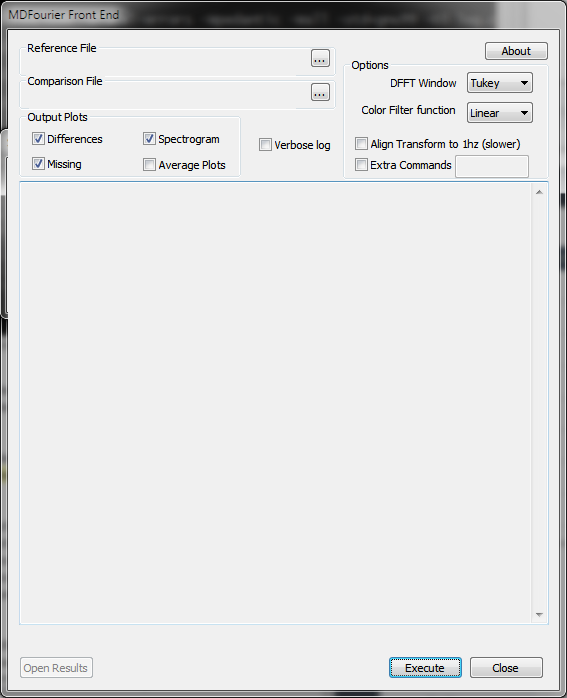
\includegraphics[width=0.6\linewidth]{plots/GUI1.png}
	\caption[Front End]{MDFourier Windows Front End}
	\label{fig:gui1}
\end{figure}

In order to generate the output plots, two files must be selected to compare them. One as a \textit{Reference} and the other as the \textit{Comparison} file as detailed in section \ref{howitworks}.

The following sequence of steps indicates the typical work flow within the GUI:

\begin{figure}[H]
	\centering
	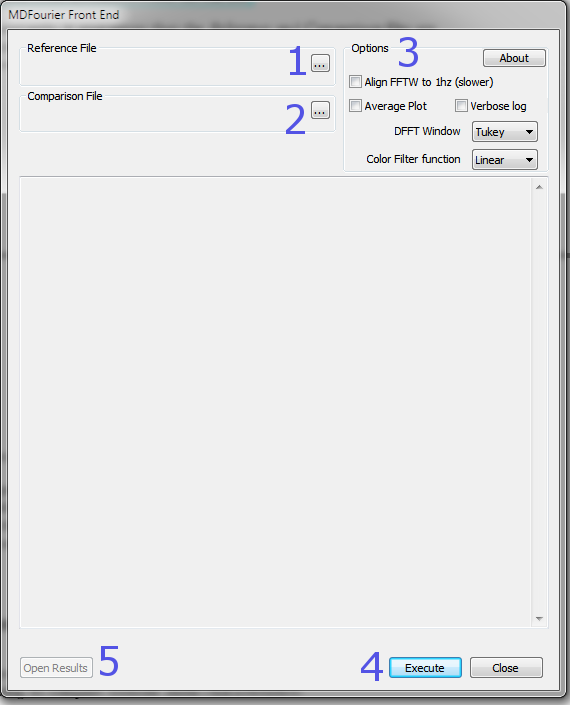
\includegraphics[width=0.6\linewidth]{plots/GUI2.png}
	\caption[Steps]{Typical sequence of steps}
	\label{fig:gui2}
\end{figure}

\begin{enumerate}
	\item Select a \textit{Reference} file
	\item Select a \textit{Comparison} file
	\item Change the default \textit{options} if needed
	\item Execute \textit{MDFourier}
	\item When execution ends, open the \textit{results folder}
\end{enumerate}

The Front End will display the output text from the command line tool, including any errors or progress available.

Keep in mind that the \textit{Open results} button will only be enabled after a successful comparison between files has been finished, and it won't open a second instance of the window if you have one already open.

\section{Front End Options}

The currently available options in the Front End are:

\begin{itemize}
	\item \textbf{DFFT Window:} In order to reduce spectral leakage a filtering window is applied to each element compared between both signals. Please consult section \ref{windows} for details. 
	\item \textbf{Color Filter Function:} This is a \textit{filter function} applied to the results in order to highlight or attenuate the differences between the files.  Please consult section \ref{colorfilter} for details. 
	\item \textbf{Align FFTW to 1hz:} Creates a version of each trimmed note, zero padded to match the sample rate in order to align the FFT bins to 1hz, as a  result there will be more dots plotted. Off by default.
	\item \textbf{Average Plot:} This traces an average line on top of the plots, making it easier to follow the data trend when the comparison file has severley scattered data. Off by default.
	\item \textbf{Verbose Log:} This option creates a detailed log in the oputput folder, useful for reporting errors or unexpected behaviour. (\textit{Please send the wav files if possible as well!})
\end{itemize}

\section{Window Functions}
\label{windows}

In order to reduce \textit{spectral leakage} a filtering window is applied to each element compared between both signals. Since we are generating the signal ourselves from the custom binary for each hardware platform, the signal can be analyzed as periodic and has a natural attack and decay rate.

By default we use a custom \textit{Tukey window} with very steep slopes. \textit{MDFourier} does offer alternate windows as options for further analysis. You can read more about windows and their usage in the reference web page\cite{windowtypes}.

\subsection{Tukey}

The default is a Tukey window specifically designed for this purpose. It uses a 2.5\% slope on each side of the signal, zeroing just a few samples and with minimal amplitude and frequency distortion.

The following equation is used to create the slopes:

\begin{equation}
tukey(x)=85(1+\cos(\frac{2\pi}{n-1}\frac{x-(n-1)}{2}))
\end{equation}

And this is the resulting plot of the Tukey window, tanges are 0-1 horizontally and -0.1 to 1.1 vertically.

\begin{figure}[H]
	\centering
	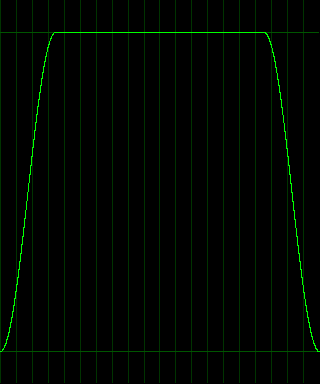
\includegraphics[width=0.4\linewidth]{plots/window-tukey.png}
	\caption[Tukey Window]{This is the custom Tukey window used by MDFourier}
	\label{fig:window-tukey}
\end{figure}


\subsection{Flattop}
A typical Flat top window is used.

\begin{align*}
flattop(x)=0.21557895 - 0.41663158\cos(2\pi\frac{x}{n-1})+ 0.277263158\cos(4\pi\frac{x}{n-1})\\
 - 0.083578947\cos(6\pi\frac{x}{n-1}) + 0.006947368\cos(8\pi\frac{x}{n-1})
\end{align*}

\begin{figure}[H]
	\centering
	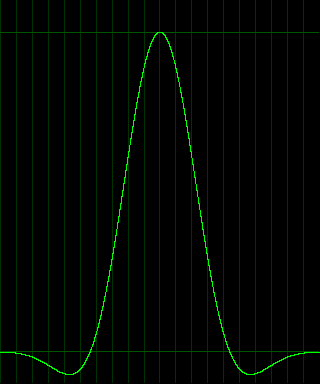
\includegraphics[width=0.4\linewidth]{plots/window-flattop.png}
	\caption[Flat Top window]{Flat Top window}
	\label{fig:window-flattop}
\end{figure}


\subsection{Hann}
A typical Hann window is used.

\begin{equation}
hann[x] = \frac{1}{2}(1 - \cos(\frac{2\pi(x+1)}{n+1}))
\end{equation}

\begin{figure}[H]
	\centering
	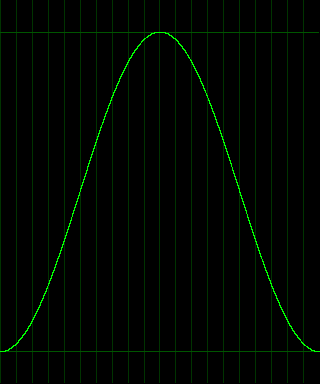
\includegraphics[width=0.4\linewidth]{plots/window-hann.png}
	\caption[Hann Window]{Hann Window}
	\label{fig:window-hann}
\end{figure}


\subsection{Hamming}
A typical Hamming window is used.

\begin{equation}
hamming[x] = 0.54 - 0.46\cos(\frac{2\pi x}{n-1})
\end{equation}

\begin{figure}[H]
	\centering
	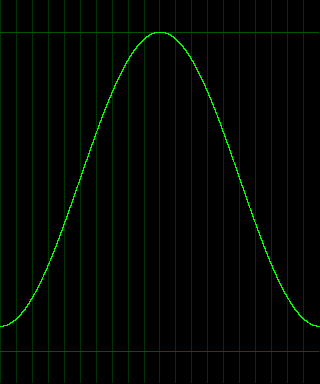
\includegraphics[width=0.4\linewidth]{plots/window-hamming.png}
	\caption[Hamming window]{Hamming window}
	\label{fig:window-hamming}
\end{figure}


\subsection{No Window}

No window is applied, equivalent to a rectangular window. This leaves the signal unprocessed and any uncontrolled decay and audio card noise will be factored in as part of the periodic signal.


\section{Color Filter Functions}
\label{colorfilter}

Each dot in the \textit{Differences} graph uses the \textit{X axis} for the frequency range and the \textit{Y axis} for the amplitude difference between the \textit{Comparison} and \textit{Reference} signals. (See section \ref{outputfiles} for output file details)

Color intensity of each dot is used to represent the amplitude for that frequency in the \textit{Reference} signal. In other words, how relevant it was to create the original signal in that note. Please refer to chapter \ref{howtoplots} in order to see examples of their use.

A color scale is presented in each graph, with the color graduation and the corresponding volume level.

\begin{figure}[H]
	\centering
	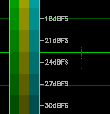
\includegraphics[width=0.2\linewidth]{plots/colorscale}
	\caption{Detail of color scale in plot}
	\label{fig:colorscale}
\end{figure}


The options are useful to highlight or attenuate these differences by applying the range to one of the following functions. 

They are sorted in descending order. The topmost option will highlight all differences; and the bottom one will attenuate most of them, and show just the ones with highest amplitudes in the \textit{Reference} signal.

\subsection{None} 

No filtering is applied, as a result all differences are plotted with the brightest color. 

\begin{figure}[H]
	\centering
	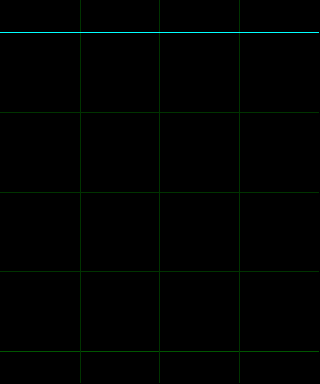
\includegraphics[width=0.4\linewidth]{plots/BetaFunctionPlot_0}
	\caption[No Filter]{No Filter}
	\label{fig:betafunctionplot0}
\end{figure}

\begin{figure}[H]
	\centering
	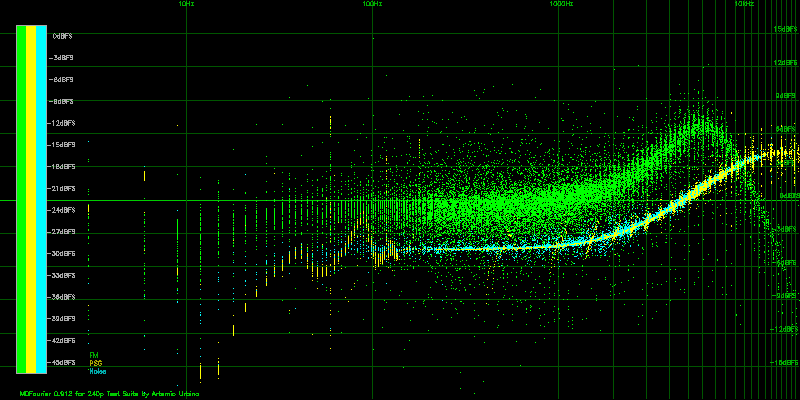
\includegraphics[width=1\linewidth]{plots/BetaFunctionPlot_0_Data}
	\caption[No Filter]{No Filter Applied}
	\label{fig:betafunctionplot0data}
\end{figure}

\newpage
\subsection{$\sqrt{dbFS}$} 

A square root function will only attenuate the lowest amplitude differences.

\begin{figure}[H]
	\centering
	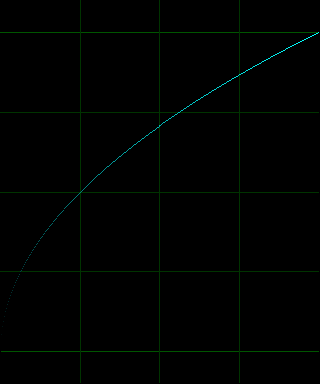
\includegraphics[width=0.4\linewidth]{plots/BetaFunctionPlot_1}
	\caption[Square Root filter]{Square Root filter}
	\label{fig:betafunctionplot1}
\end{figure}

\begin{figure}[H]
	\centering
	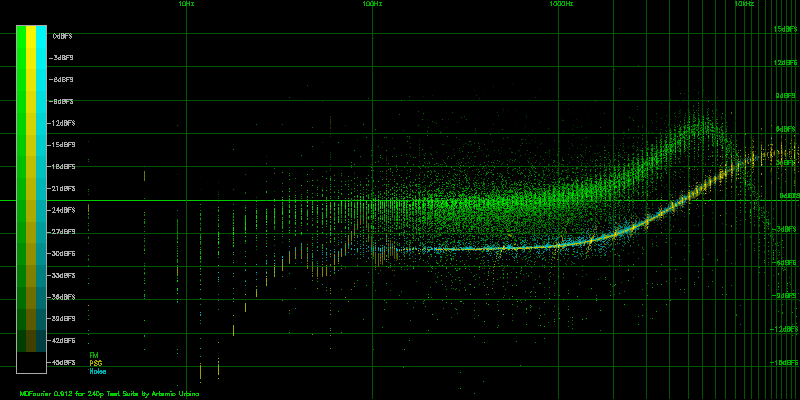
\includegraphics[width=1\linewidth]{plots/BetaFunctionPlot_1_Data}
	\caption[Square Root filter]{Square Root filter Applied}
	\label{fig:betafunctionplot1data}
\end{figure}

\newpage
\subsection{$\beta(3,3)$}

A Beta Function filter with parameters (3, 3) will attenuate a bit more from the lower range, still showing most of the differences.

\begin{figure}[H]
	\centering
	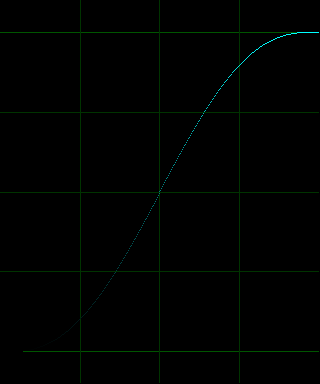
\includegraphics[width=0.4\linewidth]{plots/BetaFunctionPlot_2}
	\caption[Beta Function(3,3)]{Beta Function(3,3)}
	\label{fig:betafunctionplot2}
\end{figure}

\begin{figure}[H]
	\centering
	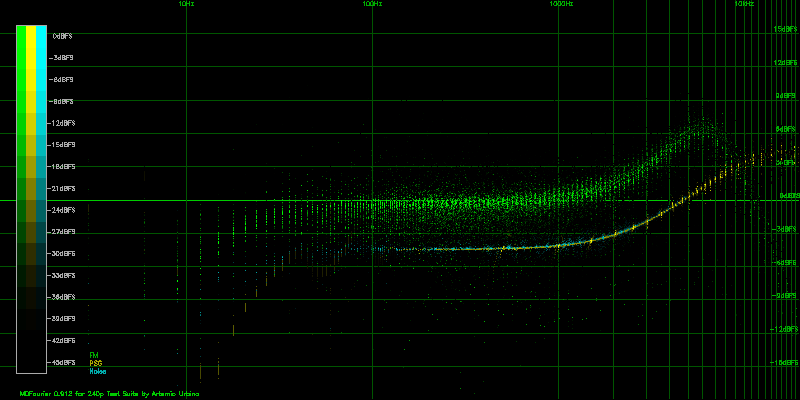
\includegraphics[width=1\linewidth]{plots/BetaFunctionPlot_2_Data}
	\caption[Beta Function(3,3)]{Beta Function(3,3) Applied}
	\label{fig:betafunctionplot2data}
\end{figure}

\newpage
\subsection{$Linear$} 

The linear function is the default, and has no bias. Half the dinamic range corresponds to half the color rage.

\begin{figure}[H]
	\centering
	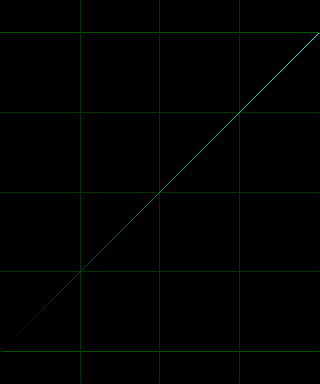
\includegraphics[width=0.4\linewidth]{plots/BetaFunctionPlot_3}
	\caption[Linear]{Linear Function}
	\label{fig:betafunctionplot3}
\end{figure}

\begin{figure}[H]
	\centering
	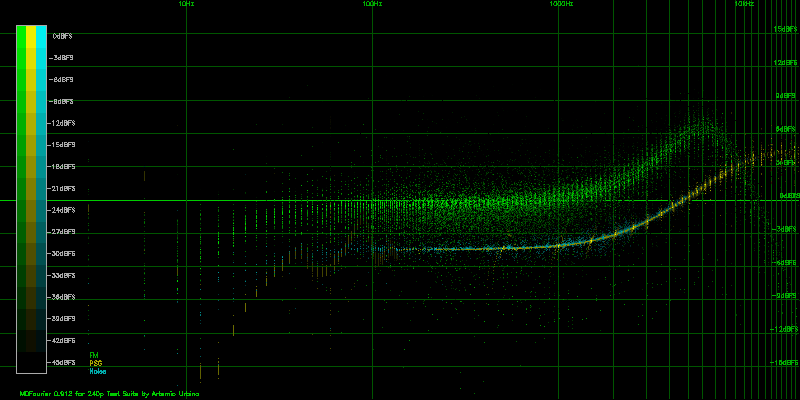
\includegraphics[width=1\linewidth]{plots/BetaFunctionPlot_3_Data}
	\caption[Linear Applied]{Linear Function Applied}
	\label{fig:betafunctionplot3data}
\end{figure}

\newpage
\subsection{$dBFS^2$}

A squared function will attenuate a lot more differences, as a result frequencies with the highest amplitude in the reference signal will be brighter.

\begin{figure}[H]
	\centering
	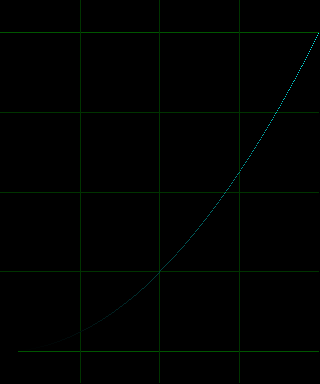
\includegraphics[width=0.4\linewidth]{plots/BetaFunctionPlot_4}
	\caption[Linear]{Linear Function}
	\label{fig:betafunctionplot4}
\end{figure}

\begin{figure}[H]
	\centering
	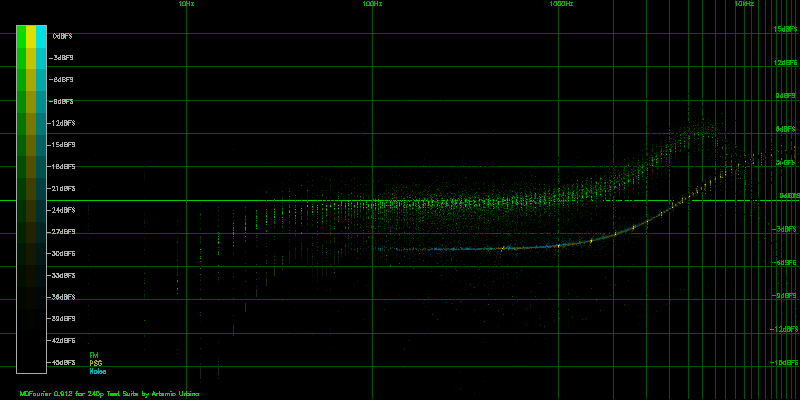
\includegraphics[width=1\linewidth]{plots/BetaFunctionPlot_4_Data}
	\caption[Linear Applied]{Linear Function Applied}
	\label{fig:betafunctionplot4data}
\end{figure}

\newpage
\subsection{$\beta(16,2)$} 

A Beta Function filter with parameters (16,2) will attenuate almost all the differences, and only the frequencies with the highest amplitude in the reference signal will be brighter.

\begin{figure}[H]
	\centering
	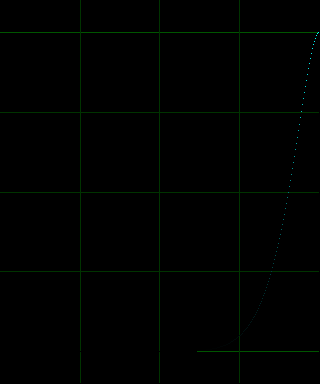
\includegraphics[width=0.4\linewidth]{plots/BetaFunctionPlot_5}
	\caption[Beta Function(16,2)]{Beta Function(16,2)}
	\label{fig:betafunctionplot5}
\end{figure}

\begin{figure}[H]
	\centering
	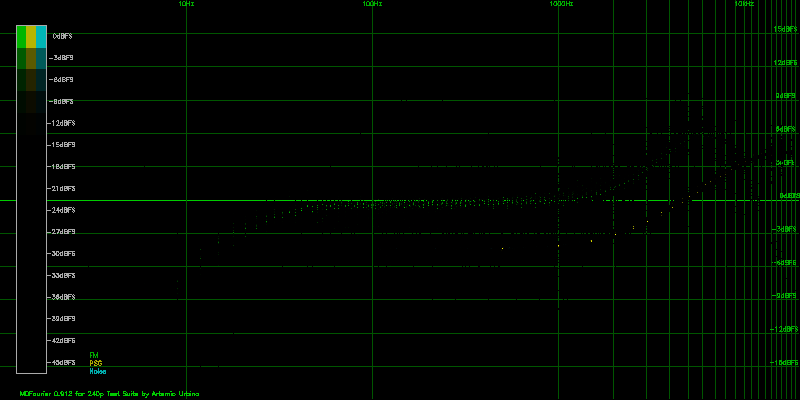
\includegraphics[width=1\linewidth]{plots/BetaFunctionPlot_5_Data}
	\caption[Beta Function(16,2)]{Beta Function(16,2) Applied}
	\label{fig:betafunctionplot5data}
\end{figure}

\chapter{How to interpret the plots}
\label{howtoplots}

The main output of the program is a set of different graphics that vary in quantity based on the definitions made in the \textit{mfn} file detailed in section \ref{mfnconfig}.

In its current form for the \textit{Mega Drive/Genesis}, there are three \textit{active blocks}: \textit{FM}, \textit{PSG} and \textit{Noise}. These will result in a plot of each type, and a general plot, being generated as output.

The files are saved under the folder \textit{MDFourier} and a sub-folder named after the input \textit{WAV} file names. They are stored in \textit{PNG}\cite{libpng} format, currently \textit{1600x800} plots are used, although this can be dynamic. 

For the current document \textit{800x400} plots were used in order to fit within a \textit{PDF} or \textit{HTML} presentation.

\section{Output Files}
\label{outputfiles}
There are common features here that we'll describe. First the type of output files: 

\begin{itemize}
	\item \textbf{DifferentAmplitude:} Plots the amplitude difference for the frequencies common to both files
	\item \textbf{MissingFrequencies:} Plots the frequencies available in the \textit{Reference} file but not found in the \textit{Comparison} file within the significant volume range.
	\item \textbf{Spectrogram:} Plots all the frequencies available in each file. Two sets of spectrograms are generated, one for the \textit{Reference} file and one for the \textit{Comparison} file.
\end{itemize}

As mentioned above, there will be several plots of each type in the output folder. One for each type, and one that summarizes all types in a single plot.

In our current\textit{ Mega Drive/Genesis} scenario, we'll get four plots of each type: \textit{FM}, \textit{PSG}, \textit{Noise} and a general one, named \textit{ALL}.

We'll follow a series of results from differen input files to MDFourier, starting with cases that have either none or a few differences, and build on top of each one so you can familiarize with what to expect as output.

\section{Scenario 1: Comparing the same file against itself}

The first scenario we'll cover is the basic one, the same file against itself. Let's keep in mind that \textit{MDFourier} is designed to show the relative differences between two audio files.

So, what is the expected result of comparing a file to itself? No differences at all, an empty plot file as shown below.

\begin{figure}[H]
	\centering
	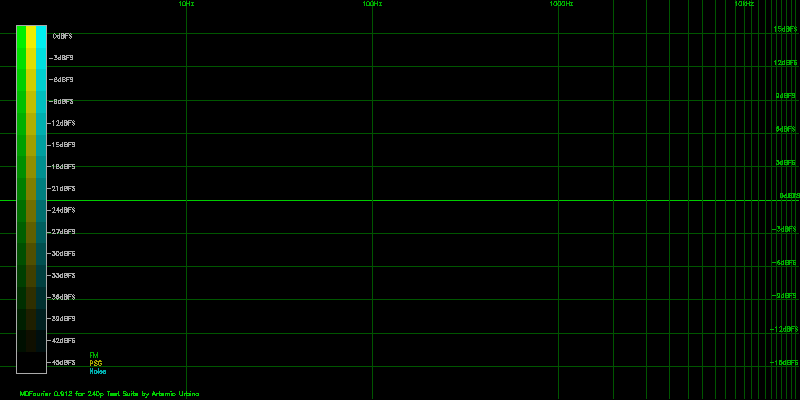
\includegraphics[width=1.0\linewidth]{plots/Plot1-SameFile.png}
	\caption[Same file compared]{Different Amplitudes result file when comparing the same file against itself.}
	\label{fig:plot1-samefile}
\end{figure}

Of course all of the \textit{Differences} and \textit{Missing} plots will only have the grid and reference bars, with no plotted information since both input files are identical. 

However there will be two sets of \textit{Spectrograms}, one for the \textit{Reference} file and one for the \textit{Comparison} file, with one plot for each type plus the general one.

\begin{figure}[H]
	\centering
	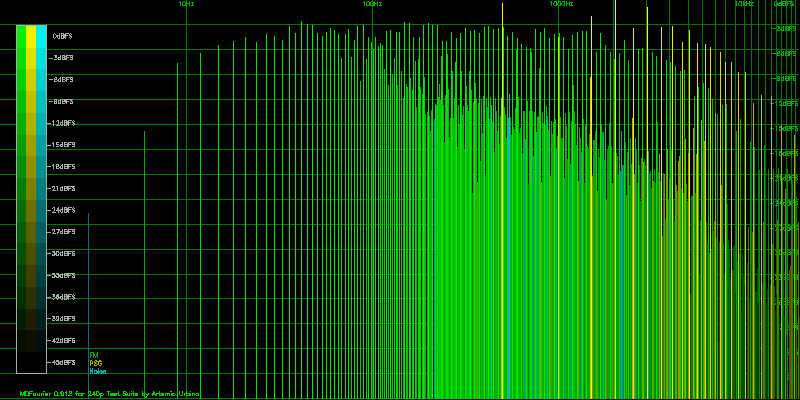
\includegraphics[width=1.0\linewidth]{plots/Plot2-SameFile-FM-Spectrogram.png}
	\caption[Spectrogram]{The Spectrogram for a Genesis 1 VA3 via hedphone out}
	\label{fig:plot2-samefile-fm-spectrogram}
\end{figure}

The Amplitude, or volume, of each of the fundamental sine waves that compose the original signal is represented by vertical lines that reach from the bottom to the point that represents the amplitude in \textit{dBFS}\cite{dbfs}. The line is also colored to represent that amplitude with the scale on the left showing the equivalence.

Three colors as defined from the \textit{mfn file} are used to plot the graph, with each one of them plotting the frequencies from each corresponding block from the \textit{WAV} file.

The top of the plot corresponds to the maximum possible amplitude, which is \textit{0 dBFS}. the bottom of the plot corresponds to the \textit{minimum significant volume}, as described in section \ref*{MinSigVolume}.

Both sets of spectrograms in this case are identical as expected. 

\section{Scenario 2: Comparing two different recordings from the same console}

This is another control case, what should we expect to see if we record two consecutive audio files from the same exact game console using the same sound card?

\begin{figure}[H]
	\centering
	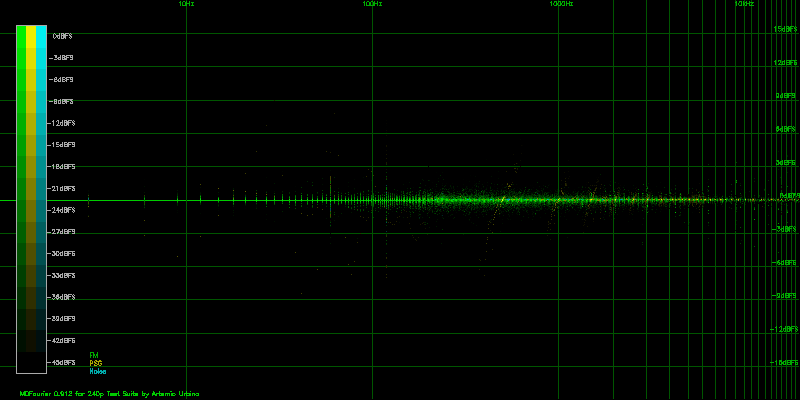
\includegraphics[width=1\linewidth]{plots/Plot2-Sameconsole}
	\caption{}
	\label{fig:plot2-sameconsole}
\end{figure}

As you can see, we have basically a flat line around zero. This means that there were no meaningful differences found. 

But wait, there are differences. Why is that? Due to many reasons: analogue recordings are not always the same for one. Then we have variations from the analogue part of console itself, and probably from the internal states and clocks from the digital side. It can also be noise generated by differences in frequency bins when performing the \textit{FFTW} after calculating the frame rates, we have that $\sfrac{1}{4}$ error after all.

We now know that there will be certain fuzziness, or variation, around each plot due to this subtle recording and performance nuances. It is a normal situation that is to be expected, and a baseline for future results.

\section{Scenario 3: Comparing against a modified file}

For demonstration purposes, the same \textit{Reference} file was modified to add a \textit{1khz 6 dbs} parametric equalization across all the analyzed signal. This is a controlled scenario to demonstrate what the plots mean.

\begin{figure}[H]
	\centering
	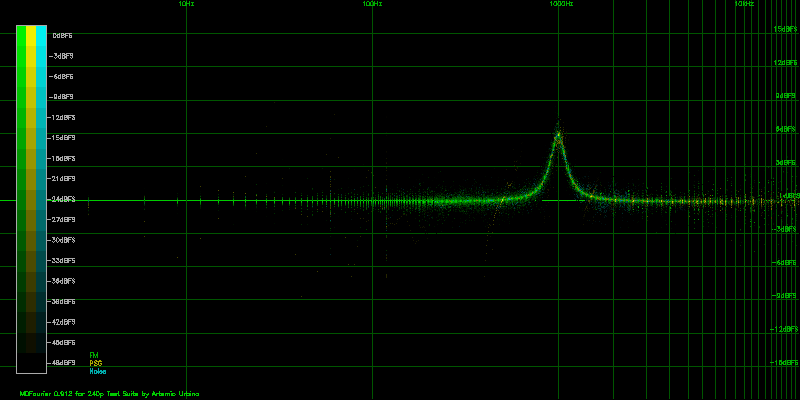
\includegraphics[width=1.0\linewidth]{plots/Plot3-Modified}
	\caption[1khz modified]{Compared against itself modified with a 1khz 6 db equalization}
	\label{fig:plot3-modified}
\end{figure}

As expected all three blocks (\textit{FM}, \textit{PSG} and \textit{Noise}) were affected and show a spike, exactly \textit{6 dBFS} tall and centered around \textit{1khz}.

It is interesting to note both spectrograms, since the \textit{1khz} spike is also shown there.

\begin{figure}[H]
	\centering
	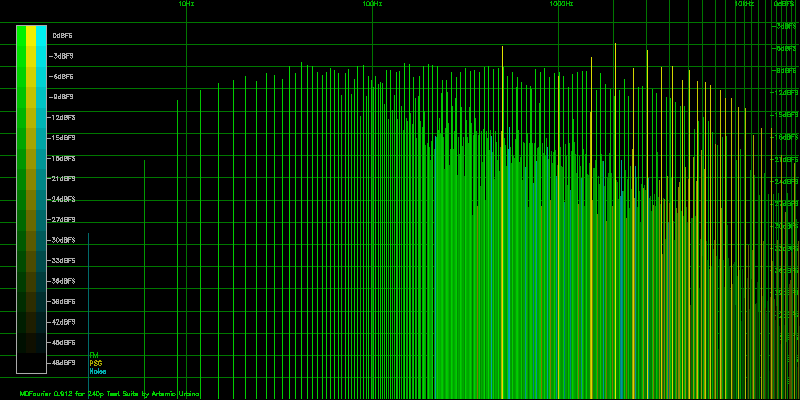
\includegraphics[width=1.0\linewidth]{plots/Plot3-Spectrogram}
	\caption[Reference File]{\textit{Reference} File}
	\label{fig:plot3-spectrogram}
\end{figure}

\begin{figure}[H]
	\centering
	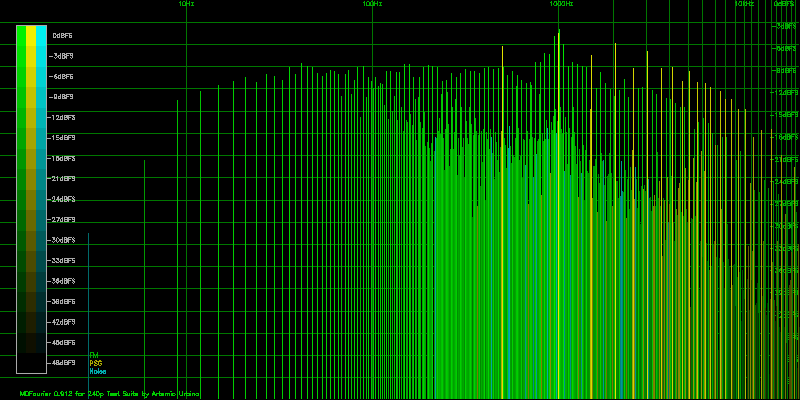
\includegraphics[width=1.0\linewidth]{plots/Plot3-Spectrogram-1khz}
	\caption[Reference File]{\textit{Reference modified with 1khz} File}
	\label{fig:plot3-spectrogram-1khz}
\end{figure}


And the \textit{Missing Frequencies} plots are basically empty, since no relevant frequencies are missing from the \textit{Comparison} file.

\section{Scenario 4: Comparing against a digital low pass and high pass filter}

We'll use the same \textit{Reference} file, and compare it to a file with a several filters:

\begin{itemize}
	\item A \textit{low pass filter} to the \textit{FM} section of the file
	\item A steeper \textit{low pass filter} at a different cutoff frequency to the \textit{PSG} section
	\item A \textit{high pass filter} to the Noise section at a different frequency
\end{itemize}

This is the general plot with the three sections:

\begin{figure}[H]
	\centering
	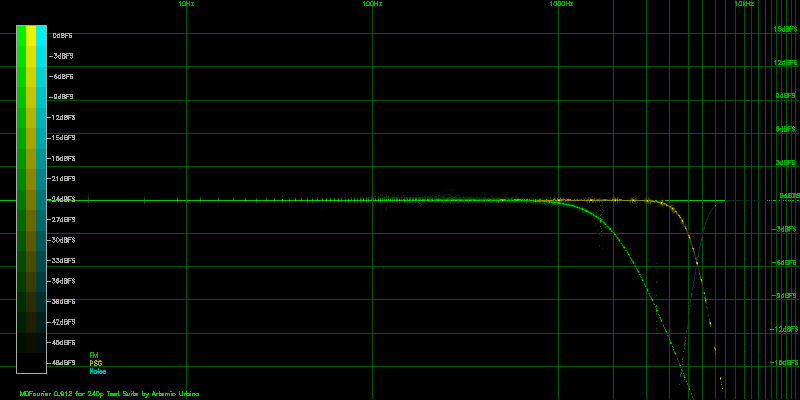
\includegraphics[width=1.0\linewidth]{plots/Plot4-1-All}
	\caption[All Plotted]{\textit{FM}, \textit{PSG} and \textit{Noise} with low pass, low pass and high pass filters.}
	\label{fig:plot4-1-all}
\end{figure}

We can now see that the higher frequencies above \textit{1khz} in the FM plot steeply go to \textit{$-\infty$ dBFS}, so the first low pass filter is there.

The second low pass filter for \textit{PSG} is at \textit{3khz}, and is steeper.

But we can barely see what is going on with the \textit{Noise} part of the plot. We can see that there is some black dots on top of the \textit{0dBFS} line.

In order to better see what is going on, we'll change the \textit{color filter function} to $\sqrt{dbFS}$ so we can have a higher contrast. (see section \ref{colorfilter})

\begin{figure}[H]
	\centering
	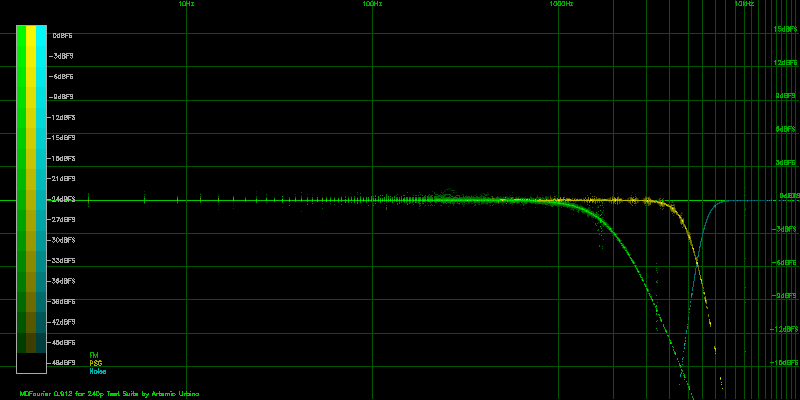
\includegraphics[width=1.0\linewidth]{plots/Plot4-2-All-sqrt}
	\caption[Using SQRT]{Using the $\sqrt{dbFS}$ color filter function}
	\label{fig:plot4-2-all-sqrt}
\end{figure}

With the higher contrast, we can now make out the curve that raises from \textit{$-\infty$ dBFS} to \textit{0 dBFS}, and it aligns with \textit{8khz}.

We can still do a little bit better, by using the \textit{Average Plot} option. (see section \ref{usinggui})

Here is the resulting plot for only the \textit{Noise} section of the signal with average enabled:

\begin{figure}[H]
	\centering
	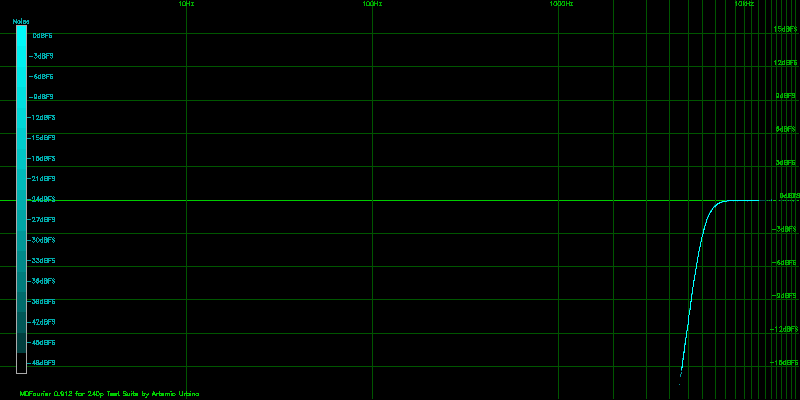
\includegraphics[width=1.0\linewidth]{plots/Plot4-3-AVG-Noise}
	\caption[Noise Average]{\textit{Noise} plot with Average}
	\label{fig:plot4-3-avg-noise}
\end{figure}

There are some other interesting plots that result from this experiment. For once, the \textit{Missing} plots now show all the frequencies the \textit{low/high pass} filters cut off.

\begin{figure}[H]
	\centering
	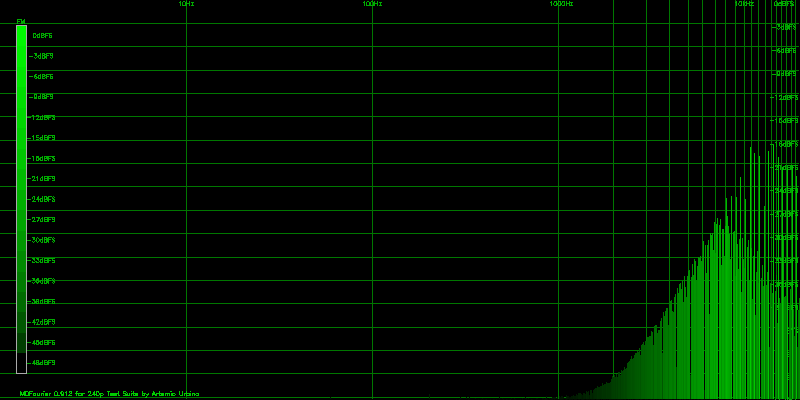
\includegraphics[width=1.0\linewidth]{plots/Plot4-4-Missing-FM}
	\caption[Missing FM]{Missing frequencies in \textit{FM} cutoff by low pass filter}
	\label{fig:plot4-4-missing-fm}
\end{figure}

As show in figure \ref{fig:plot4-4-missing-fm}, there is a curve in the spectrogram and only frequencies above \textit{1khz} show up, slowly rising in amplitude.

\begin{figure}[H]
	\centering
	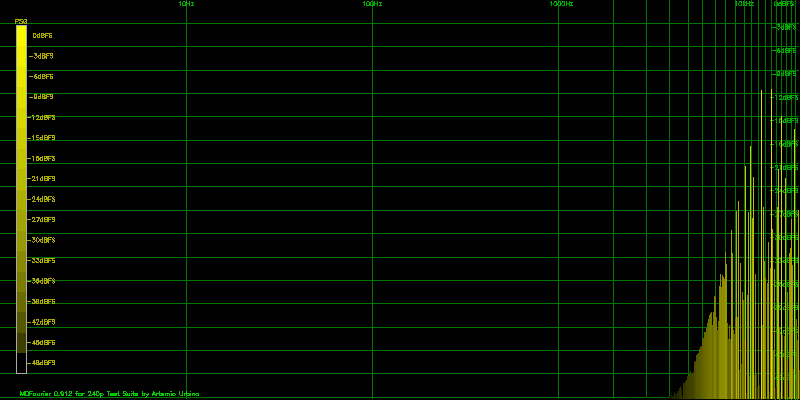
\includegraphics[width=1.0\linewidth]{plots/Plot4-5-Missing-PSG}
	\caption[Missing PSG]{Missing frequencies in \textit{PSG} cutoff by low pass filter}
	\label{fig:plot4-5-missing-psg}
\end{figure}

The same behavior can be observed in the \textit{PSG spectrogram}, but with a different curve that starts at \textit{4khz} in figure \ref{fig:plot4-5-missing-psg}.

\begin{figure}[H]
	\centering
	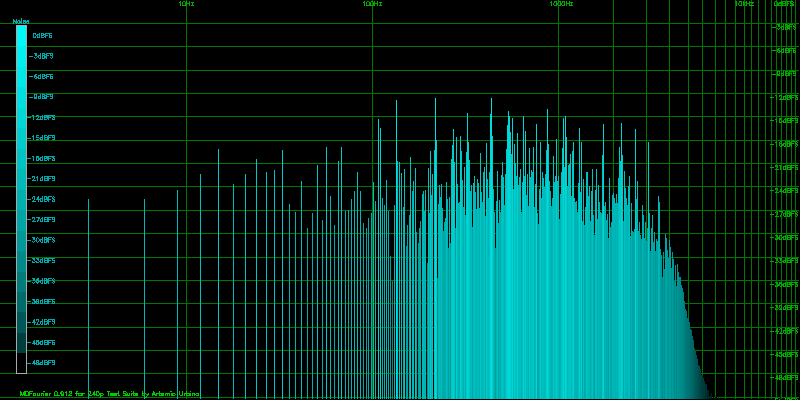
\includegraphics[width=1.0\linewidth]{plots/Plot4-6-Missing-Noise}
	\caption[Missing Noise]{Missing frequencies in \textit{Noise} cutoff by high pass filter}
	\label{fig:plot4-6-missing-noise}
\end{figure}

And finally, figure \ref{fig:plot4-6-missing-noise} shows the opposite kind of curve, the high pass filter cuts off everything higher than \textit{8khz} in the \textit{Noise} section.

It is a good moment to emphasize that these are relative plots. They show how different the \textit{Comparison} signal is to the \textit{Reference} signal. And so far we've compared the same signal to itself although modified with very precise digital manipulations. An analog filter would look the same, but a bit fuzzier. 

However, some interesting ideas arise. What would happen if we take this low/high pass filter signal and use it as \textit{Reference} and the original one as \textit{Comparison}?

\begin{figure}[H]
	\centering
	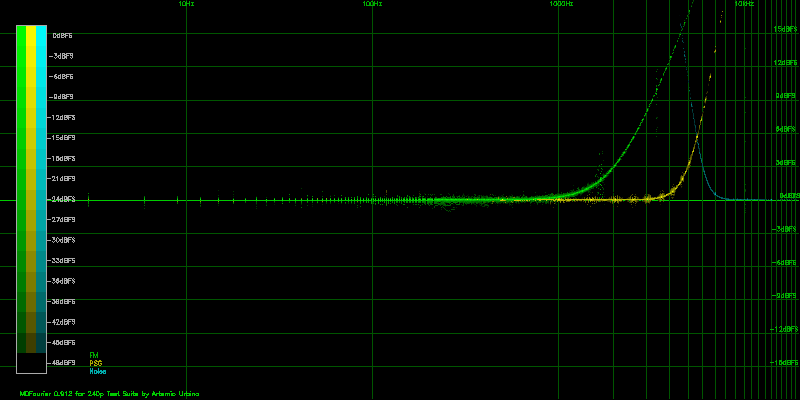
\includegraphics[width=1.0\linewidth]{plots/Plot4-7-Reversed}
	\caption[Reversed]{Results when using modified signal as \textit{Reference}}
	\label{fig:plot4-7-reversed}
\end{figure}

Based on this, one could jump to the conclusion that everything will simply be inverted. After all, the original signal not rises to \textit{$+\infty$ dBFS} at the same spots, and that makes complete sense since those frequencies have now a higher amplitude. And although the \textit{Differences} and \textit{Spectrogram} plots will indeed be inverted under these controlled conditions, the \textit{Missing} plots are different.

Most of them are now empty:

\begin{figure}[H]
	\centering
	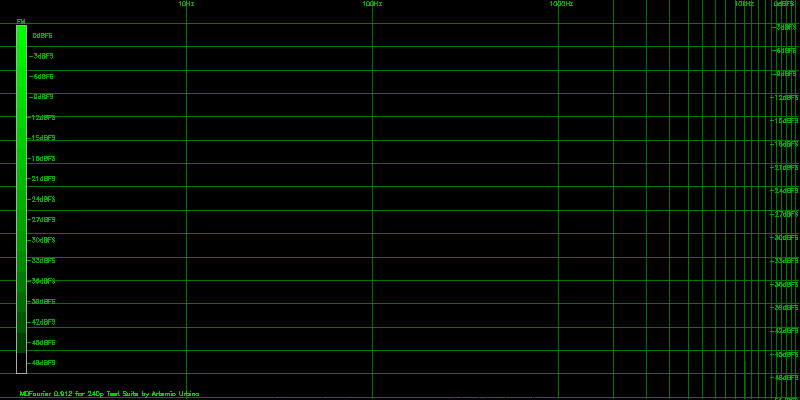
\includegraphics[width=1.0\linewidth]{plots/Plot4-8-Missing-FM-Inverted}
	\caption[Reversed FM Missing]{\textit{Missing Frequencies} plot for \textit{FM} is empty}
	\label{fig:plot4-8-missing-fm-inverted}
\end{figure}

This happens because we cut a lot of frequencies with such steep low and high pass filters, and all the frequency content from this modified signal is present in the original, but not the other way around as we saw before.

\section{Scenario 5: Comparing two recordings from the same console made with different Audio Cards}

We'll now compare the same console using two different recordings, one made with an internal \textit{PCI M-Audio 192} and the other with a \textit{USB Lexicon Alpha}. Here are the results:

\begin{figure}[H]
	\centering
	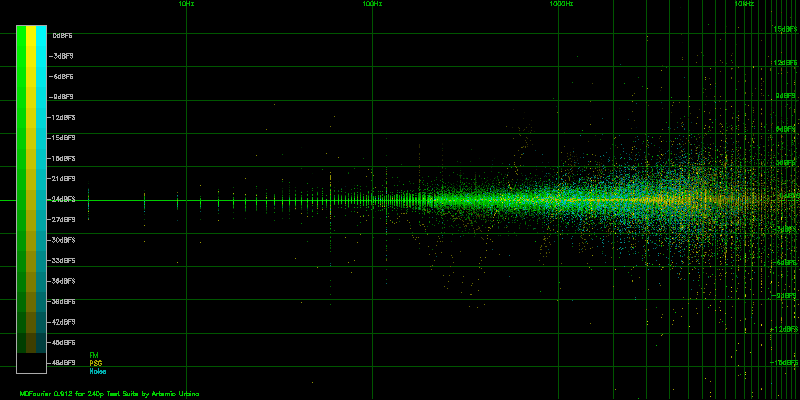
\includegraphics[width=1.0\linewidth]{plots/Plot5-1-All}
	\caption[Reversed FM Missing]{Differences using same hardware and cables, different capture cards}
	\label{fig:plot5-1-all}
\end{figure}

Well, I am guessing that was unexpected. We can tell a few things though. First, the frequency response is slightly different, since we now have that huge scatter at the higher end of the spectrum, the treble.

But we can still make out the scatter is centered around the \textit{0 dBFS} line, which means that even using different sound cards we can probably make out differences. Also, the sampling was not exactly the same with both cards, there was a slight difference in the detected frame rates:

\begin{figure}[H]
	\centering
	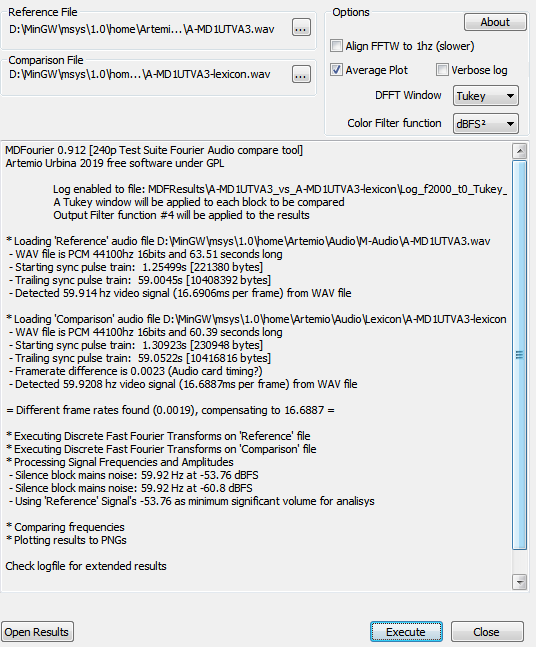
\includegraphics[width=0.6\linewidth]{plots/Plot5-1-FramerateDiff.png}
	\caption[Front End]{Frame rate difference}
	\label{fig:plot5-1-frameratediff}
\end{figure}


* Loading 'Reference' audio file
- WAV file is PCM 44100hz 16bits and 63.51 seconds long
- Starting sync pulse train:  1.25499s [221380 bytes]
- Trailing sync pulse train:  59.0045s [10408392 bytes]
- Detected 59.914 hz video signal (16.6906ms per frame) from WAV file

* Loading 'Comparison' audio file 
- WAV file is PCM 44100hz 16bits and 60.39 seconds long
- Starting sync pulse train:  1.30923s [230948 bytes]
- Trailing sync pulse train:  59.0522s [10416816 bytes]
- Detected 59.9208 hz video signal (16.6887ms per frame) from WAV file

= Different frame rates found (0.0019), compensating to 16.6887 =


Here is the graph with the \textit{Average plot} option turned on.



\chapter{Results from vintage retail hardware}

The following table lists all the hardware used to make the recordings for the plots that will be shown. All had stock parts at the time of the recording, and used original power supplies. They were all connected to a 4" \textit{CRT} via \textit{RGB}, although the \textit{CRT} was turned off while recording. Recordings were made on \textit{5/25/2019}.

\begin{center}
\scalebox{0.6}{
\begin{tabular}{ | l | l | l | l | l | l | l | l | l | }
    \hline
	Type    & Model    & Revision & FCCID & Serial & Region & Made in & MDFourier ID & Recorded from\\
    \hline
	Model 1 & HAA-2510 & VA1    &               & 89N61751  & Japan & Japan  & A-MD1JJVA1   & Headphone Out\\
	Model 1 & 1601     & VA3    & FJ846EUSASEGA & 30W59853  & USA   & Taiwan & A-MD1UTVA3   & 	Headphone Out\\
	Model 1 & 1601     & VA6    & FJ8USASEGA    & B10120356 & USA   & Japan  & A-MD1UJVA6   & Headphone Out\\
	Model 1 & 1601     & VA6    & FJ8USASEGA    & 59006160  & USA	& Taiwan & A-MD1UTVA6-1 & 	Headphone Out\\
	Model 1 & 1601     & VA6    & FJ8USASEGA    & 31X73999  & USA   & Taiwan & A-MD1UTVA6-2 & Headphone Out\\
	Model 1 & HAA-2510 & VA6    &               & A10416197 & Japan	& Japan  & A-MD1JJVA6   & Headphone Out\\
	Model 2 & MK-1631  & VA1.8  & 	FJ8MD2SEGA  & 151014280 & USA   & China  & A-MD2UCVA18  & 	AV Out\\
	Nomad   & MK-6100  &        &  50059282	    &           & USA	& Taiwan & A-NMUT       &	Headphone Out\\
	CDX     & MK-4121  &        & Y40 014198    &           & USA   & Japan  & A-CDXUJ-LO   &	Line Out\\
	CDX     & MK-4121  &        & Y40 014198    &           & USA   & Japan  & A-CDXUJ-HP   &	Headphone Out\\
	\hline
\end{tabular}
}
\end{center}

\chapter{MDWave}
\label{mdwave}

\textit{MDWave} is a companion command line tool to \textit{MDFourier}. While developing the tool suite and learning about \textit{DSP}, I needed to check what I was doing and visualise or listen to the results. Hence, \textit{MDWave} was born.

It takes a single wave file as argument, and follows all the parameters defined in the configuration file (see section \ref{mfnconfig}).

It has a few more commmand line options, which I'll detail in later versions of the document. You can type \textit{mdwave -h} in your \textit{mdfourier} folder for details.

\chapter{Compiling from source code}

\section{Dependencies}

\textit{MDFourier} needs a few libraries to be compiled. The pre-compiled binary created with \textit{MinGW}\cite{mingw} is statically linked against:

\begin{itemize}
	\item fftw-3.3.8\cite{fftw}
	\item libpng-1.5.30\cite{libpng}
	\item plotutils-2.6\cite{libplot}
	\item incbeta\cite{betafunction} (included with source code)
\end{itemize}

In \textit{Linux} or \textit{UN*X} based systems, you can link it against the latest versions or the libraries.

The \textit{makefiles} to compile either version are provided with the source code\cite{sourcecode}.

\chapter{Contact the author}
\label{contact}

You can contact me via twitter \url{http://twitter.com/Artemio} or e-mail me at \textit{aurbina@junkerhq.net}

\begin{thebibliography}{9}
	\bibitem{sourcecode}
	Github,
	\textit{MDFourier source code C99},
	\url{https://github.com/ArtemioUrbina/MDFourier}.
	
	\bibitem{maudio}
	M-Audio Audiophile 192,
	\textit{Specifications},
	\url{https://www.soundonsound.com/reviews/m-audio-audiophile-192}.
	
	\bibitem{lexicon}
	Lexicon Alpha USB card,
	\textit{Product web page},
	\url{https://lexiconpro.com/en/products/alpha}.
	
	\bibitem{240pSuite}
	240p test Suite,
	\textit{Wiki web page},
	\url{http://junkerhq.net/240p}.
	
	\bibitem{audacity}
	Audacity
	\textit{web page},
	\url{https://www.audacityteam.org/}.
	
	\bibitem{goldwave}
	Goldwave
	\textit{product web page},
	\url{https://www.goldwave.com/}.
	
	\bibitem{fftw}
	Fastest Fourier Transform in the West.,
	\textit{web page},
	\url{http://fftw.org/}.
	
	\bibitem{windowtypes}
	Window Types: Hanning, Flattop, Uniform, Tukey, and Exponential ,
	\textit{web page},
	\url{https://community.plm.automation.siemens.com/t5/Testing-Knowledge-Base/Window-Types-Hanning-Flattop-Uniform-Tukey-and-Exponential/ta-p/445063}.
	
	\bibitem{libpng}
	libPNG
	\textit{web page},
	\url{https://sourceforge.net/projects/libpng/files/libpng15/1.5.30/}
	
	\bibitem{libplot}
	GNU Plot Utils
	\textit{web page},
	\url{https://www.gnu.org/software/plotutils/}
	
	\bibitem{mingw}
	MinGW, 
	\textit{Minimalist GNU for Windows},
	\url{http://mingw.org/}.
	
	\bibitem{betafunction}
	incbeta, 
	\textit{Incomplete Beta Function in C},
	\url{https://codeplea.com/incomplete-beta-function-c}.
	
	\bibitem{dbfs}
	dB Full Scale, 
	\url{https://www.sweetwater.com/insync/dbfs/}
\end{thebibliography}

\end{document}
